\chapter{System Implementation}

This chapter presents the screenshots of the SmartSec AI-Based Cyber Defense Platform,
demonstrating the fully implemented and deployed user interface. All screens shown below
are captured from the live running application built with React 18 and Vite, connected
to the FastAPI backend and Supabase PostgreSQL database.

% ── Login / Register Page ──────────────────────────────────────────────────────
\begin{figure}[H]
    \centering
    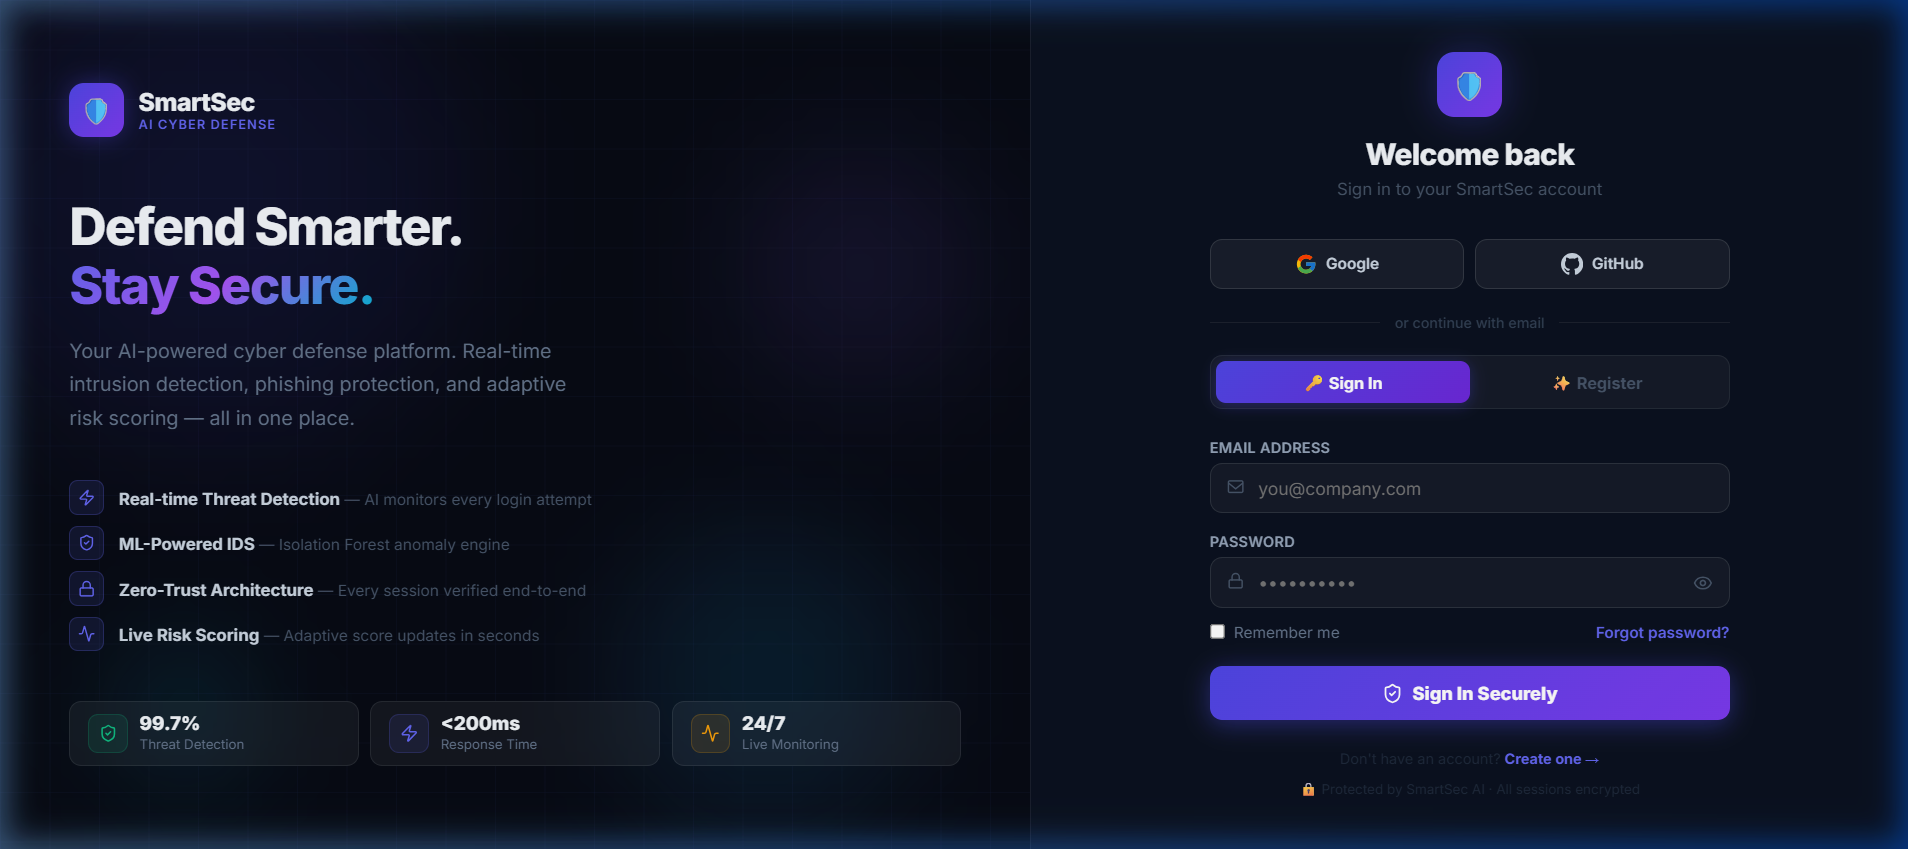
\includegraphics[width=0.90\linewidth,height=0.80\textheight,keepaspectratio]{login_page}
    \caption[]{User Authentication Page -- Login and Registration Interface}
    \label{fig:login_page}
\end{figure}
\FloatBarrier

\noindent The login page features a dark-themed glassmorphism design with dual Login and
Register tabs. The form validates email format and password length before submission.
Google and GitHub OAuth buttons are provided below the standard credentials form.

\newpage

% ── Main Dashboard ─────────────────────────────────────────────────────────────
\begin{figure}[H]
    \centering
    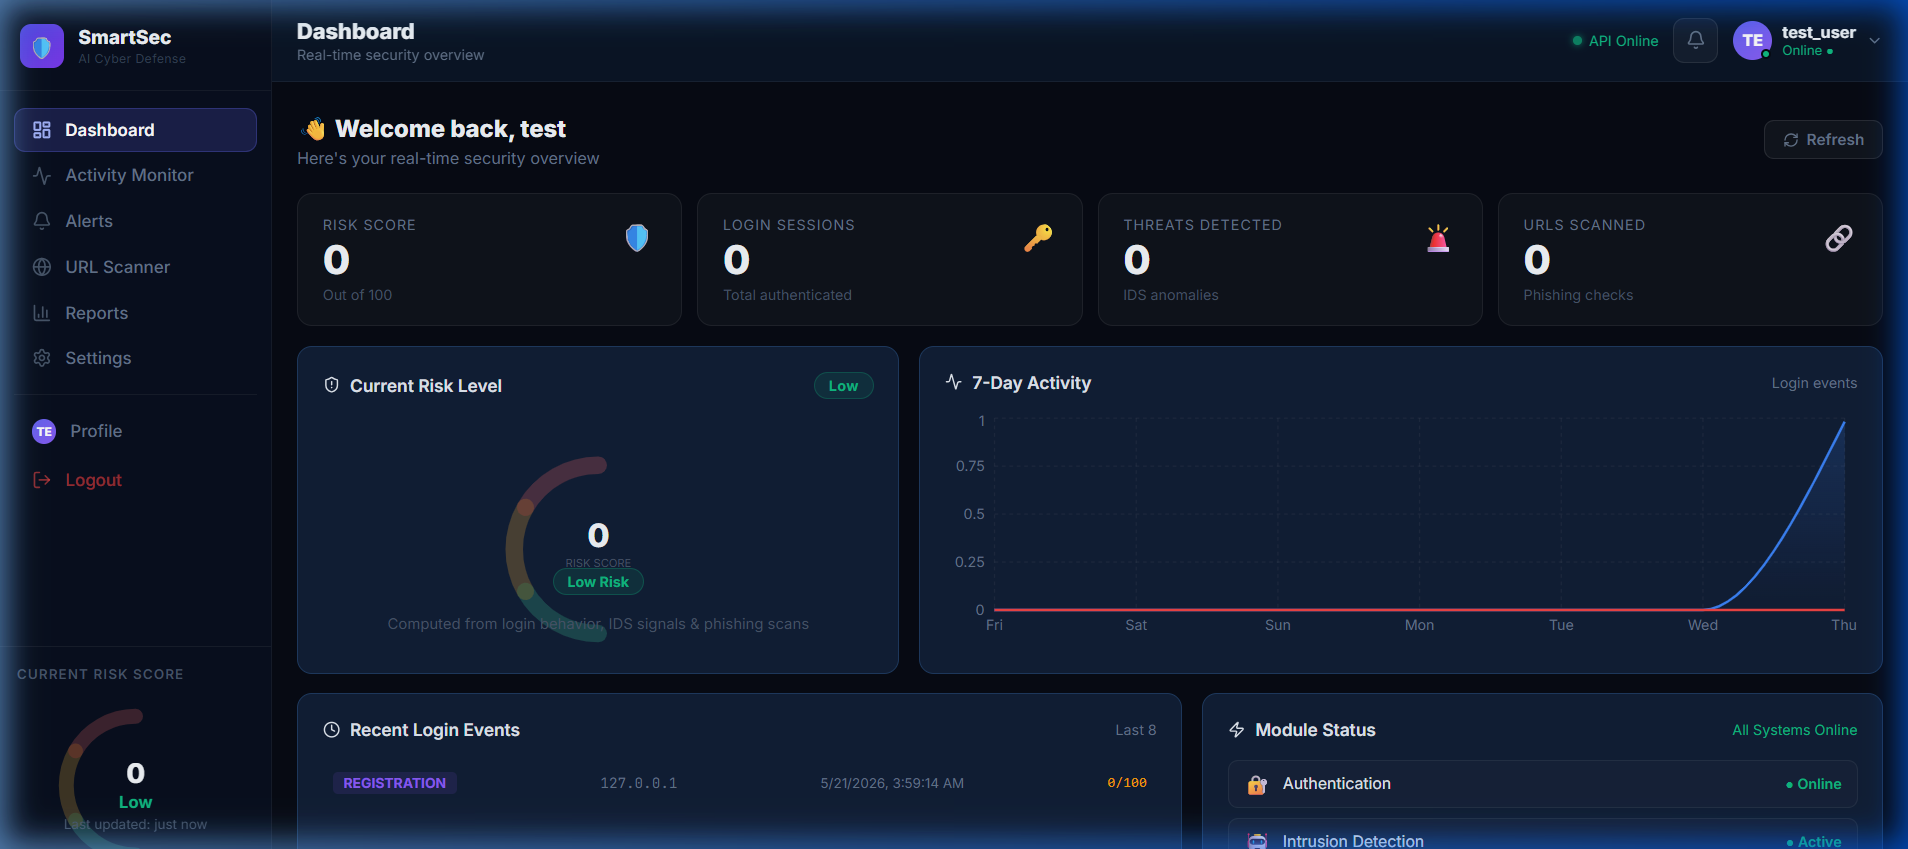
\includegraphics[width=0.90\linewidth,height=0.80\textheight,keepaspectratio]{dashboard_page}
    \caption[]{Security Dashboard -- Live Stats, Risk Level, and 7-Day Activity Chart}
    \label{fig:dashboard_page}
\end{figure}
\FloatBarrier

\noindent The main dashboard aggregates data from all security modules into a single view.
It displays metric cards showing total URL scans, phishing detections, IDS anomalies,
and the current risk level. A Recharts AreaChart shows the 7-day rolling security
activity trend. All data is fetched live from the FastAPI /dashboard endpoint on load.

\newpage

% ── IDS Anomaly Detection ──────────────────────────────────────────────────────
\begin{figure}[H]
    \centering
    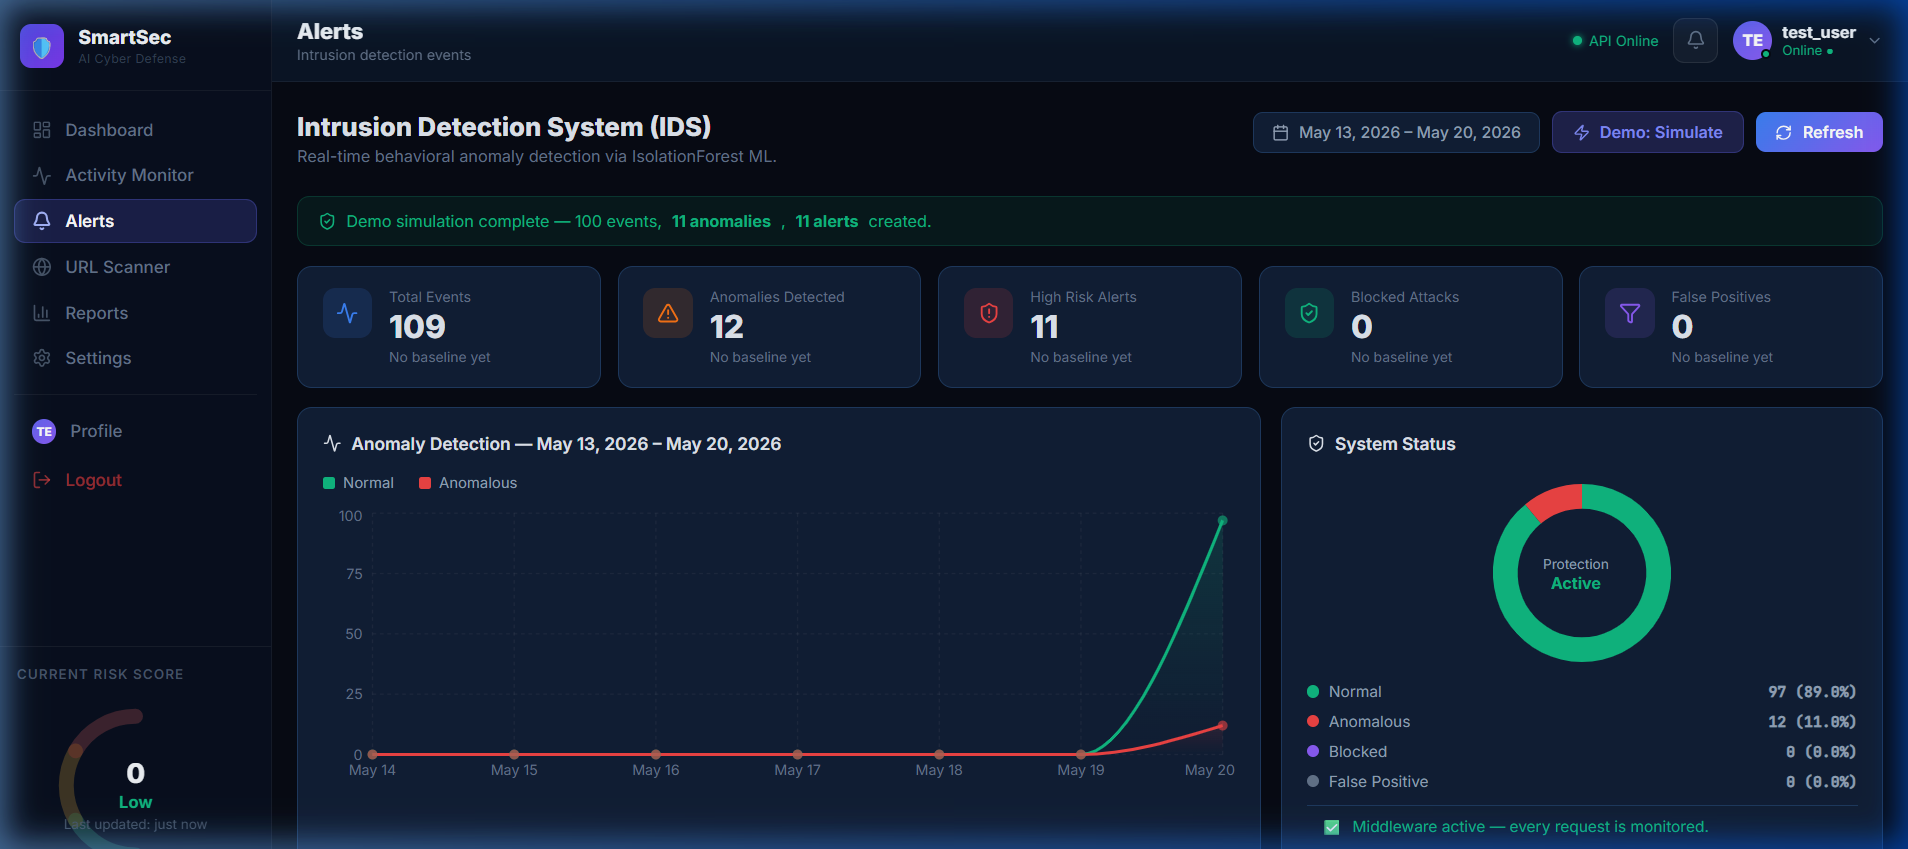
\includegraphics[width=0.90\linewidth,height=0.80\textheight,keepaspectratio]{ids_page}
    \caption[]{IDS Module -- IsolationForest Anomaly Detection and Traffic Simulation}
    \label{fig:ids_page}
\end{figure}
\FloatBarrier

\noindent The IDS page allows users to trigger synthetic traffic simulation through the
IsolationForest ML model. The results show the count of normal sessions versus anomalies
detected, an anomaly rate percentage, a distribution pie chart, and a table of recent
anomaly records with timestamps, feature values, and confidence scores.

\newpage

% ── Phishing URL Scanner ───────────────────────────────────────────────────────
\begin{figure}[H]
    \centering
    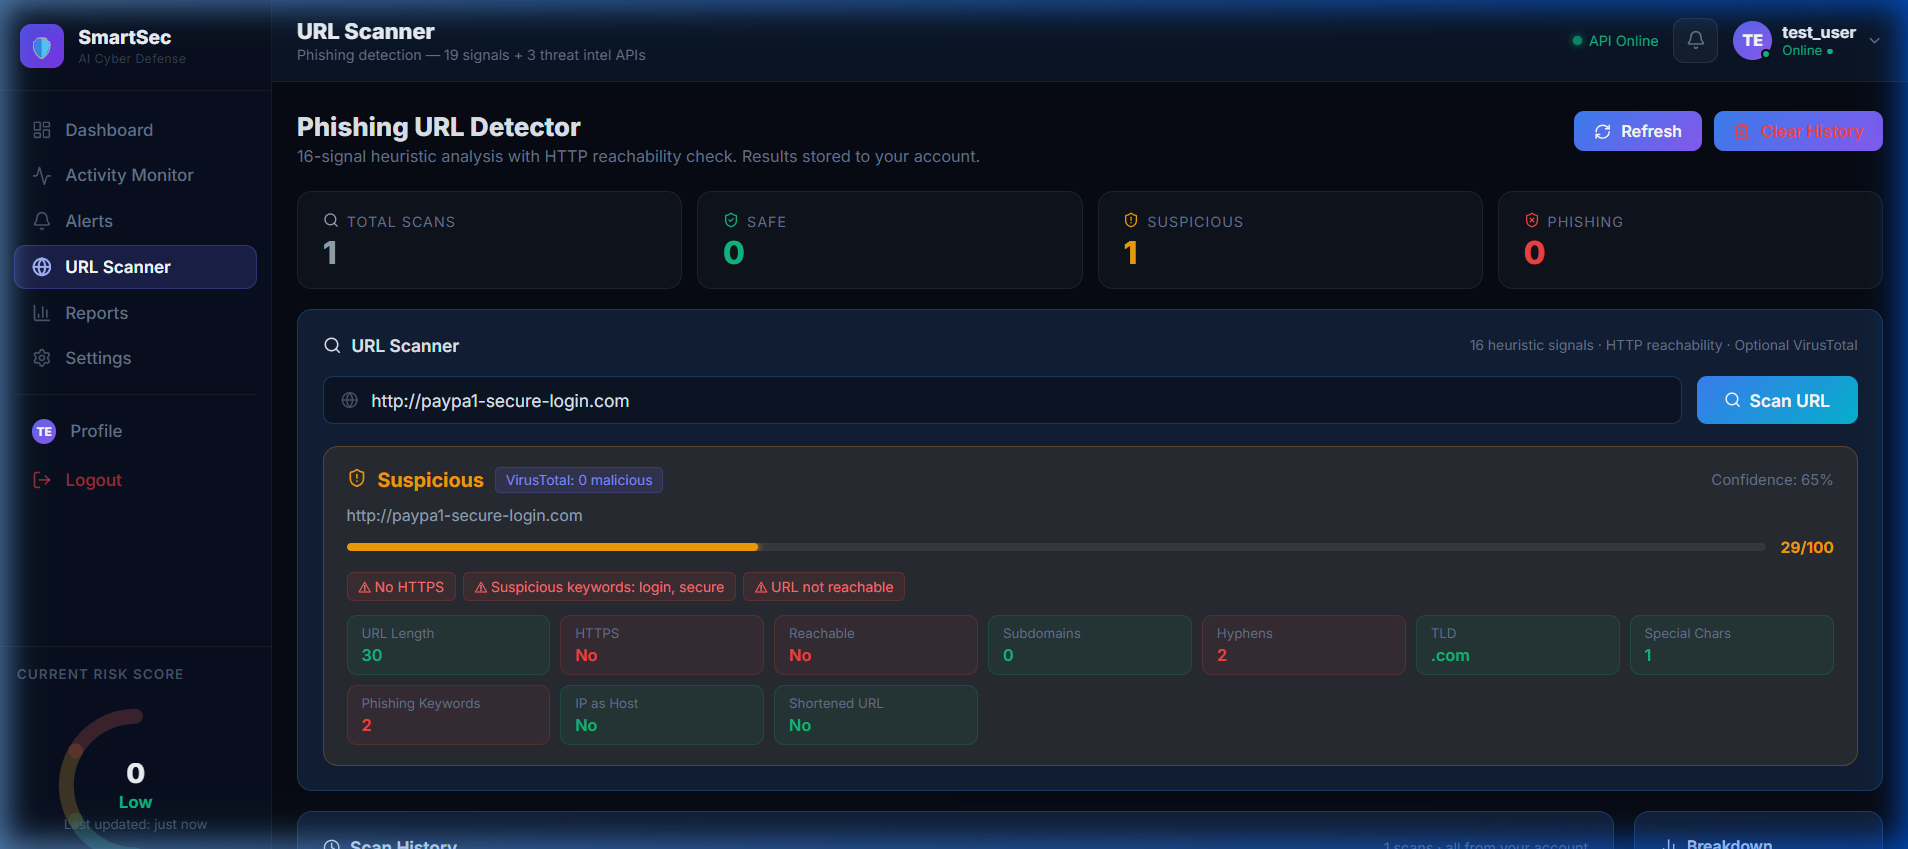
\includegraphics[width=0.90\linewidth,height=0.80\textheight,keepaspectratio]{phishing_page}
    \caption[]{Phishing URL Scanner -- Multi-API Verdict, Risk Score, and Signal Breakdown}
    \label{fig:phishing_page}
\end{figure}
\FloatBarrier

\noindent The phishing scanner accepts any URL input and performs a 19-signal heuristic
analysis combined with VirusTotal, Google Safe Browsing, and AbuseIPDB API lookups.
The result panel shows the final verdict (Safe / Suspicious / Phishing), overall risk
score, confidence percentage, and a complete breakdown of which signals were triggered.
Scan history is maintained in a paginated table below the scanner.

\newpage

% ── Risk Score Engine ─────────────────────────────────────────────────────────
\begin{figure}[H]
    \centering
    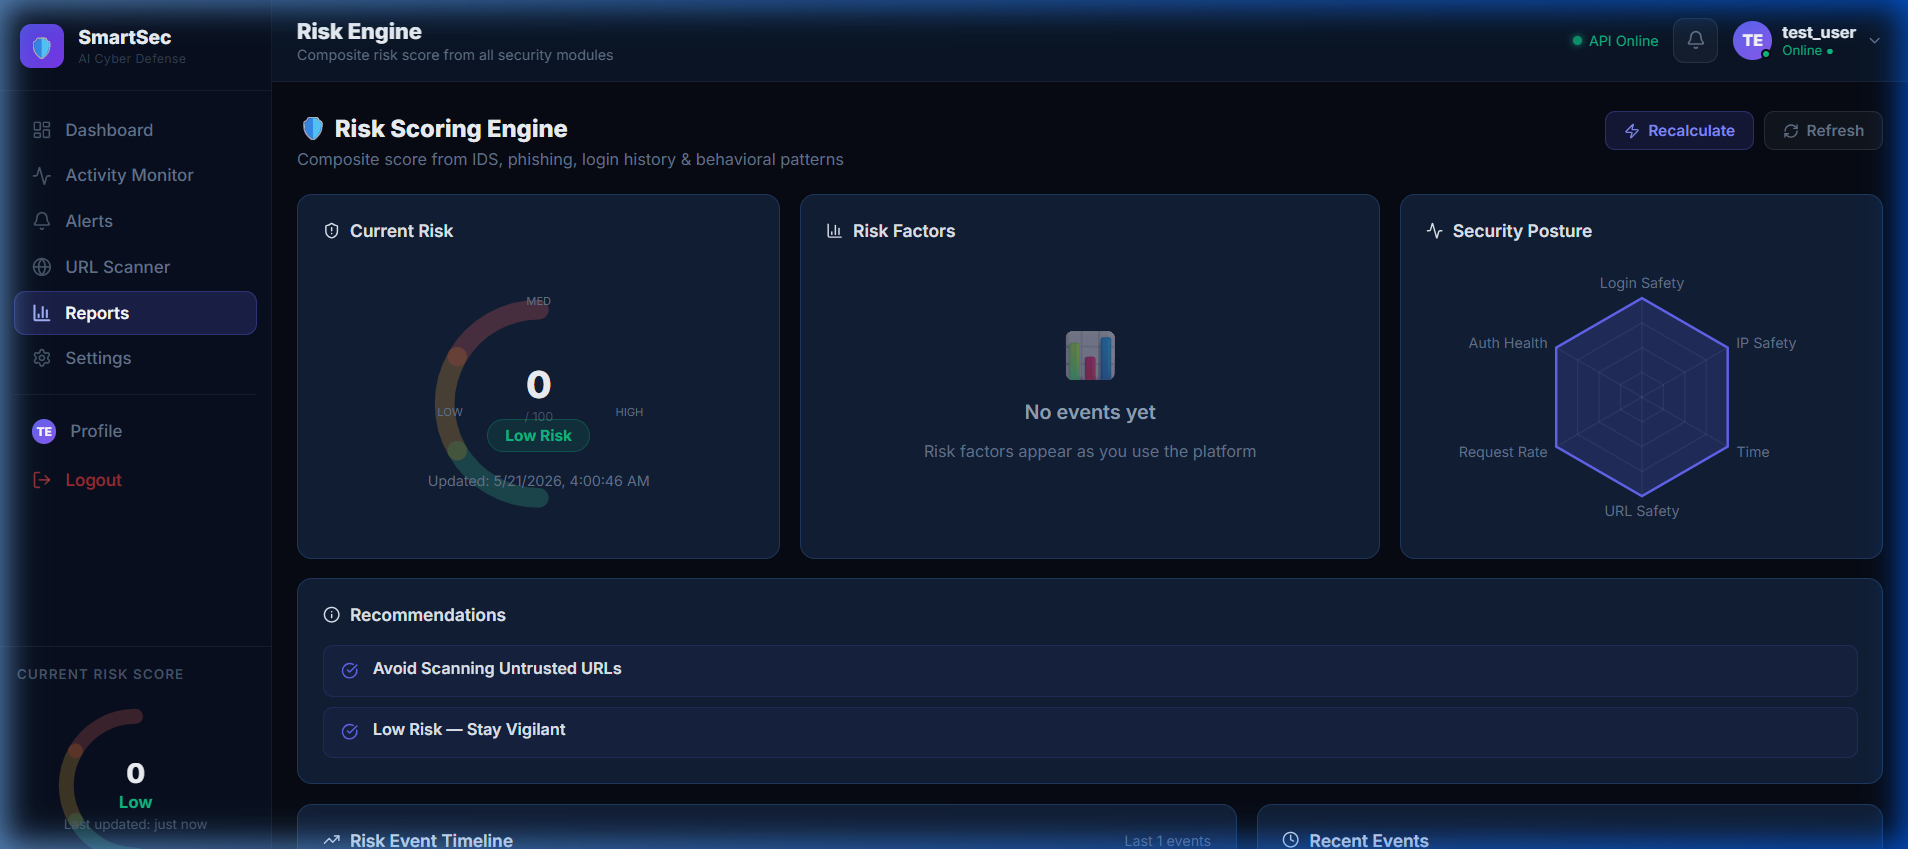
\includegraphics[width=0.90\linewidth,height=0.80\textheight,keepaspectratio]{risk_page}
    \caption[]{Risk Scoring Engine -- Score Gauge, Category Breakdown, Event Timeline, and Recommendations}
    \label{fig:risk_page}
\end{figure}
\FloatBarrier

\noindent The risk page presents the user's current security posture score (0--100) on a
visual gauge with colour-coded zones (Green / Yellow / Orange / Red). Below the gauge,
a Recharts RadarChart shows the risk distribution across categories (Authentication,
Network, Web, Data, System). A chronological event timeline lists all risk events with
their severity and score deltas, and an AI-generated recommendations panel suggests
specific remediation actions based on the current risk profile.

\newpage

% ── Activity Monitor ──────────────────────────────────────────────────────────
\begin{figure}[H]
    \centering
    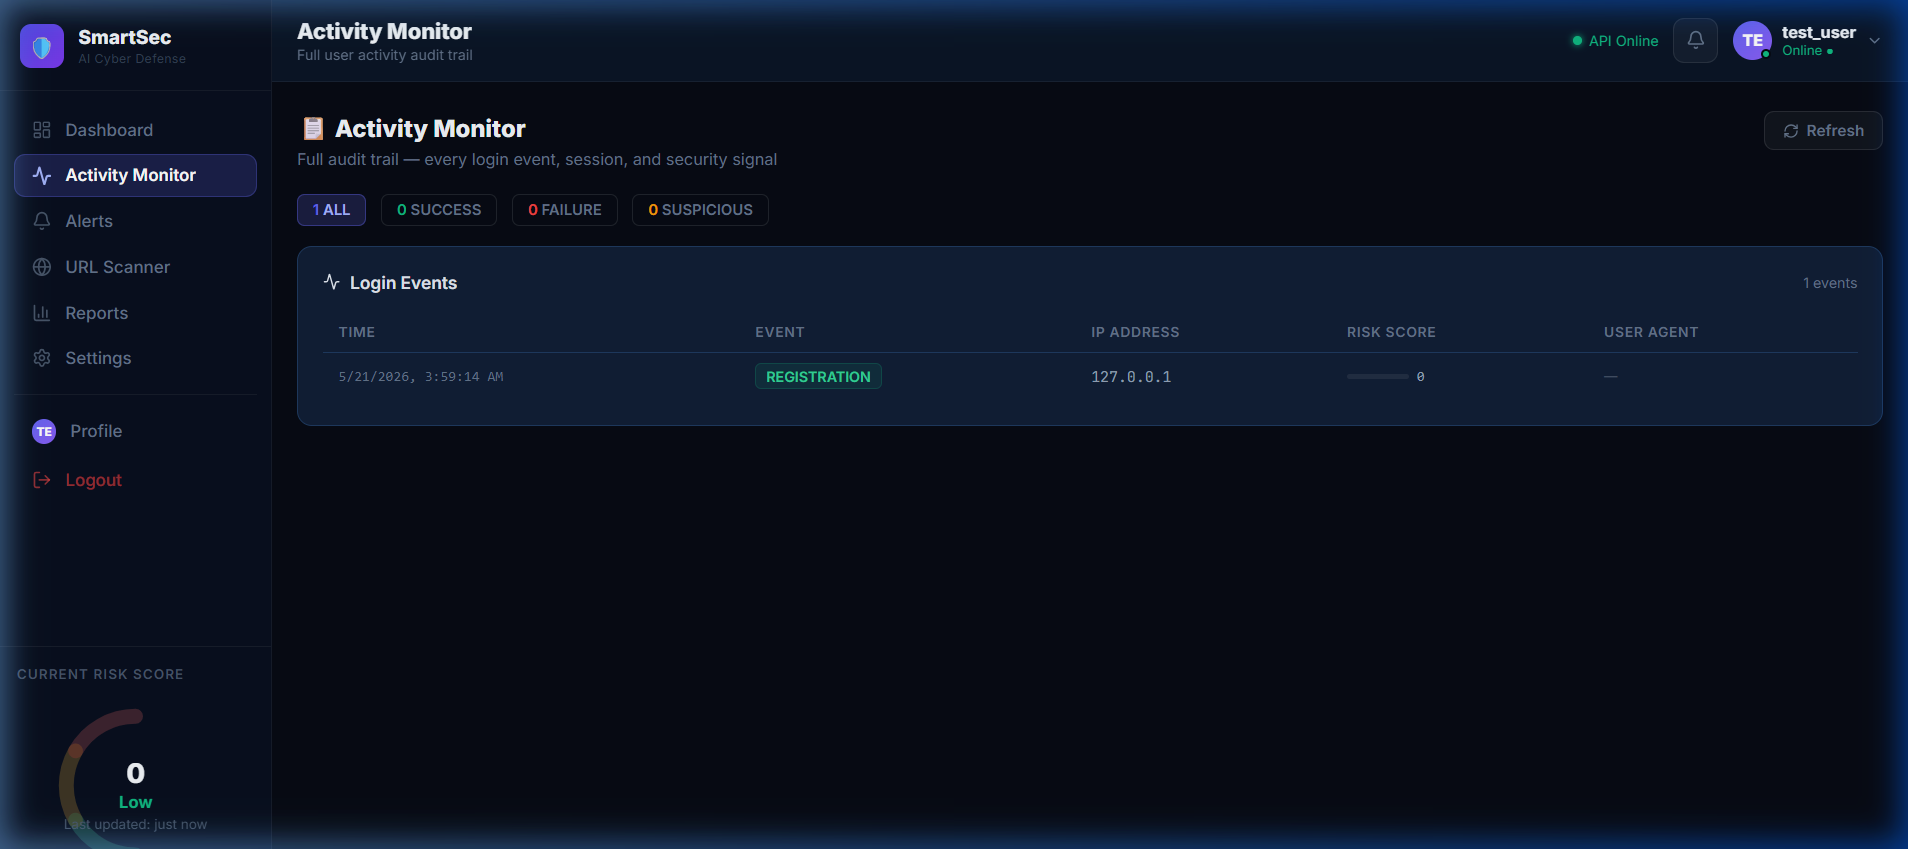
\includegraphics[width=0.90\linewidth,height=0.80\textheight,keepaspectratio]{activity_page}
    \caption[]{Activity Monitor -- Complete Login Audit Trail with IP Address and Risk Flags}
    \label{fig:activity_page}
\end{figure}
\FloatBarrier

\noindent The Activity Monitor provides a full audit trail of every authentication event
for the account. Each entry records the event type (Login Success, Failure, Suspicious),
timestamp, source IP address, and any risk flags triggered (off-hours access, new IP,
high failure count). This module enables forensic review of account access history and
supports incident investigation.

\newpage

% ── User Profile Page ─────────────────────────────────────────────────────────
\begin{figure}[H]
    \centering
    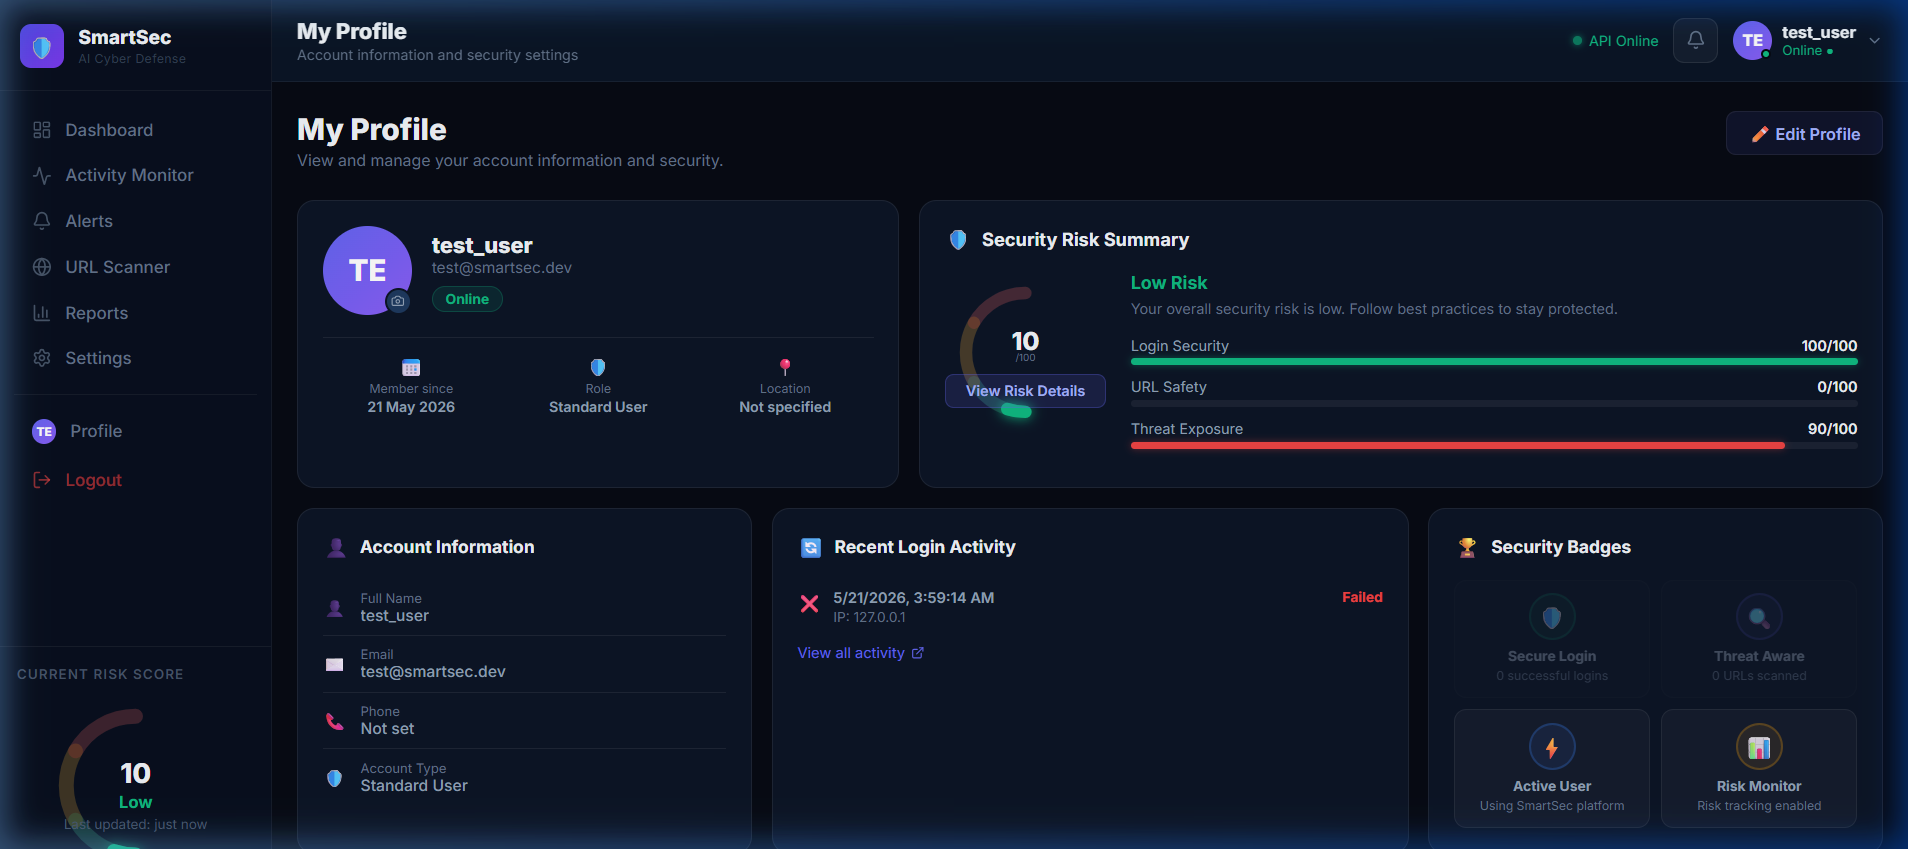
\includegraphics[width=0.90\linewidth,height=0.80\textheight,keepaspectratio]{profile_page}
    \caption[]{User Profile Page -- Account Details, Avatar, and Security Statistics}
    \label{fig:profile_page}
\end{figure}
\FloatBarrier

\noindent The profile page allows users to view and update their account information
including full name, bio, location, and phone number. An avatar upload feature supports
custom profile pictures stored in Supabase Storage. The profile card also displays a
live security summary including current risk level, total scans performed, and account
creation date.

\newpage

% ── Settings Page ─────────────────────────────────────────────────────────────
\begin{figure}[H]
    \centering
    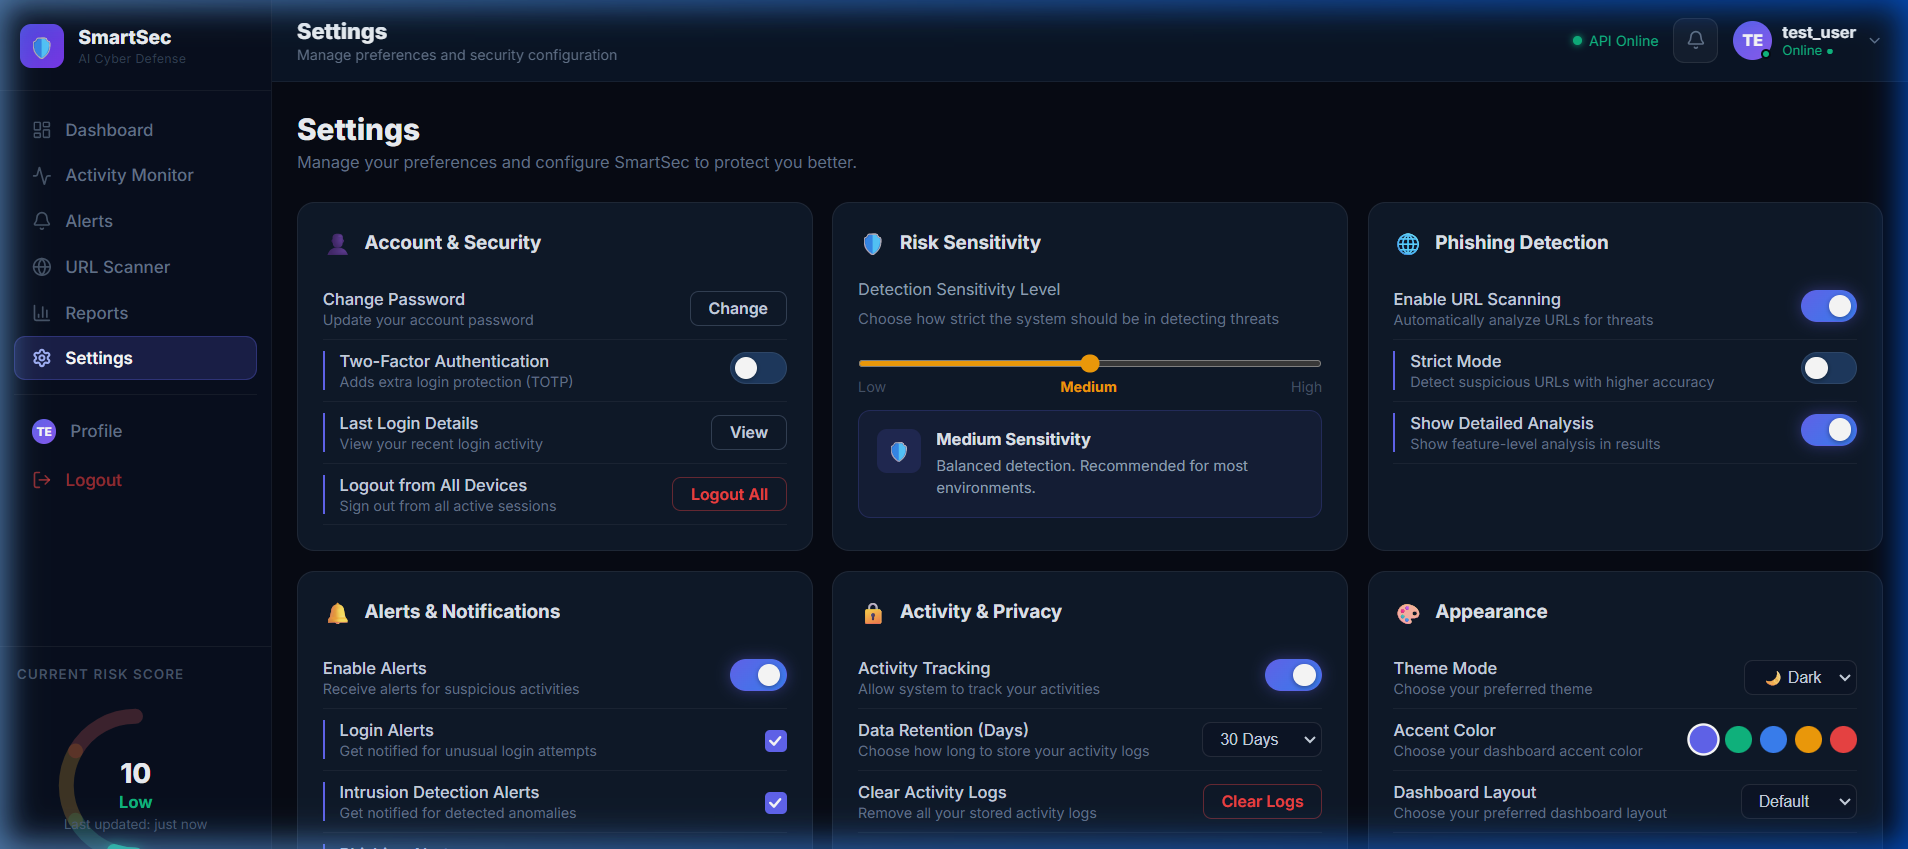
\includegraphics[width=0.90\linewidth,height=0.80\textheight,keepaspectratio]{settings_page}
    \caption[]{Security Settings Page -- Notification Preferences and Threshold Configuration}
    \label{fig:settings_page}
\end{figure}
\FloatBarrier

\noindent The settings page enables users to configure their security preferences,
including email alert thresholds, notification preferences for each event type, and
account security settings such as changing the password and activating two-factor
authentication. All settings are persisted to the JSONB user\_settings field in
the Supabase users table and applied to subsequent risk scoring and alerting logic.
